\subsection{Implementaion of Lexer and Parser}
Now that we have written the lexer and parser rules 
using ANTLR format, we can run our files against 
ANTLR and get our parser in the desired target 
language that we want. Before that, to use testing 
tools, we can compile our grammar with the java and 
see that it gives us the desired AST by using the 
graphical representation of the tree against some 
valid inputs in the DOT language. Before that, the 
installation of things that is needed is shown on this 
website \href{https://www.antlr.org/index.html}{\textbf{here}}. 
After that, you can get the parse tree for the specificed input with these commands:
\begin{lstlisting}[ style=mystyle]
$ antlr4 *.g4 -o test
$ javac DOT*.java
$ grun DOT graph
> digraph G {
> subgraph cluster0 {
> style=filled;
> a0 -> a1;
> label = "1";
> }
> subgraph cluster1 {
> node [style=filled];
> b0 -> b1 -> b2 -> b3;
> label = "2";
> }
> start -> a0;
}
\end{lstlisting}
Lines proceded by \$ are commands and lines proceded by
> are input. The output parse tree is shown in Figure \ref{fig:parse-tree}.

\begin{figure}[H]
\centering
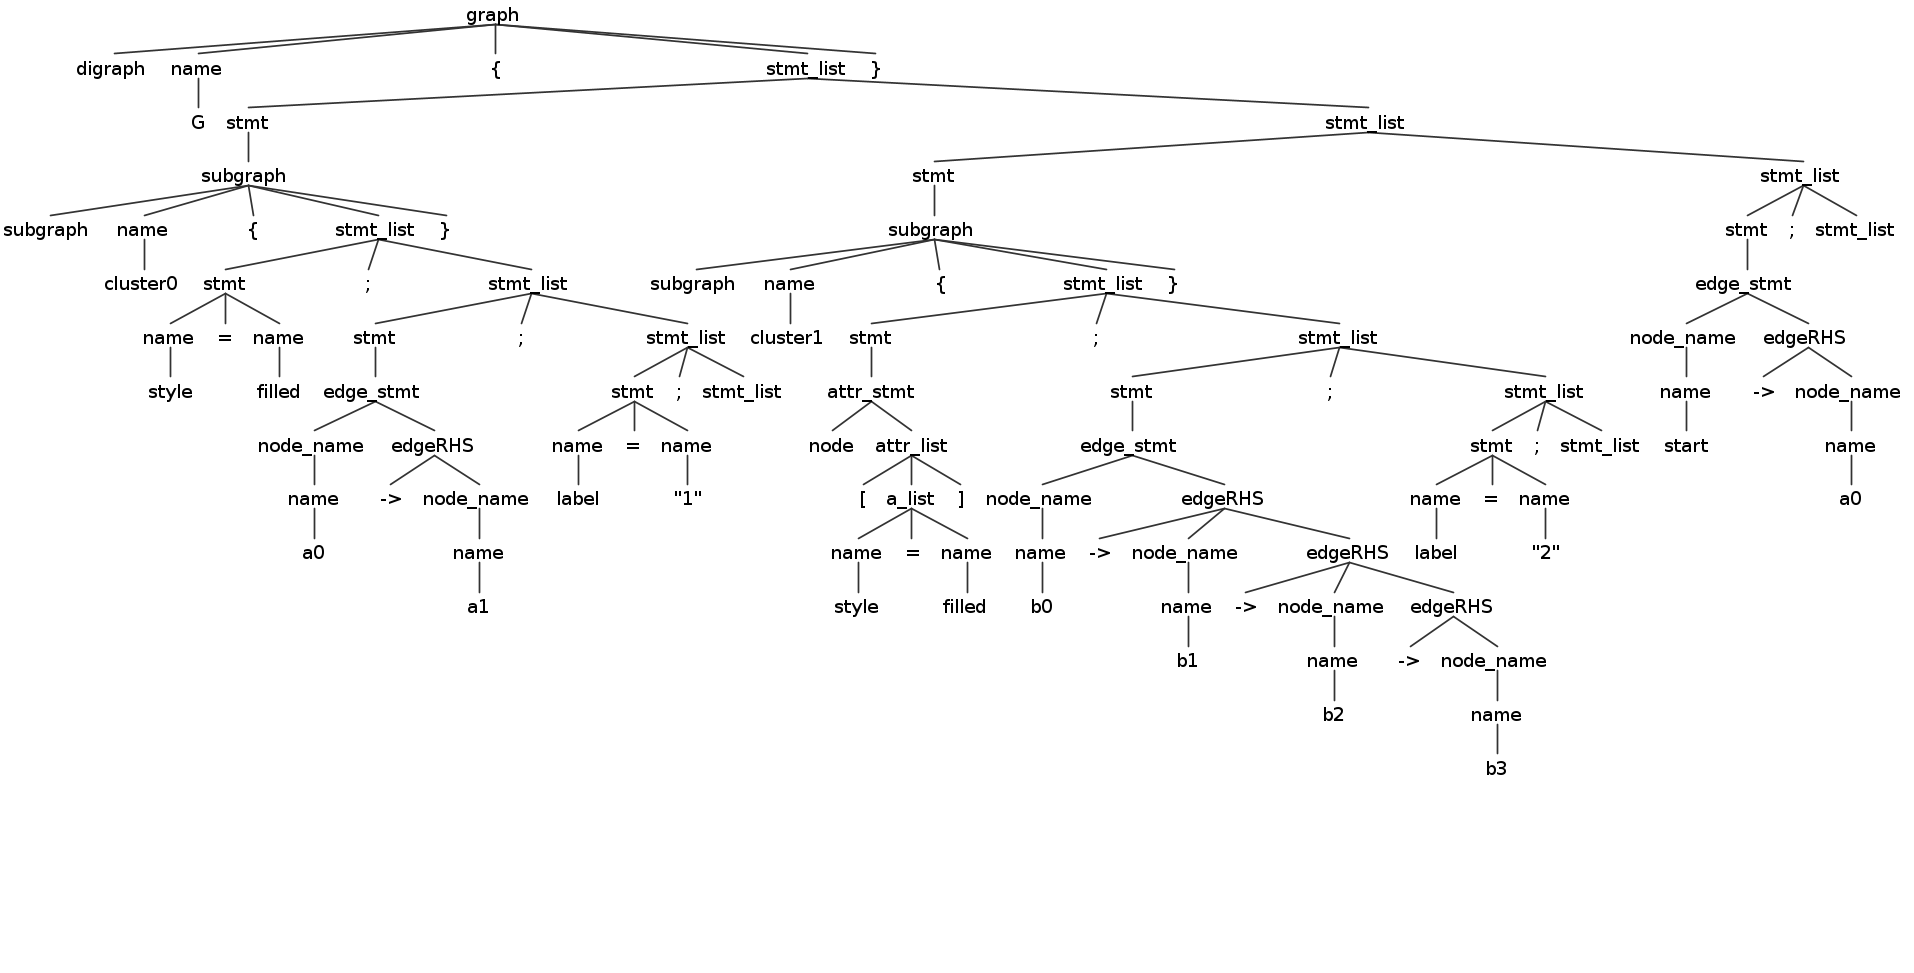
\includegraphics[width=\linewidth]{images/parse-tree.png}
\caption{Parse tree picture of the Above commands.}
\label{fig:parse-tree}
\end{figure}